\chapter{Antenna calculation and simulations}
In this thesis, the chosen transceiver has a operating frequency range from 2400 to 2525MHz, this means that when calculating and simulating the antennas, it is easier to go with a fixed frequency, therefore the center frequency will be used which is 2463MHz or 2463.000.000Hz.

By using the electromagnetic waves function the wavelength can be derived:

\begin{equation}
  f = \frac{c}{\lambda}
\end{equation}

Where f is frequency in Hz, c is the speed of light in meters m/s and $\lambda$ is the wavelength in meters m. 

Wavelength is:

\begin{equation}
  \lambda = \frac{c}{f} \Rightarrow \lambda = \frac{299782458 [m/s]}{2.463.000.000 [Hz]} = 0.1217 meters
\end{equation}

\section{4NEC2}
As explained in the introduction, the 4NEC2 program is made by a radio amateur named Arie Voors\cite{4nec2}, with the goal of being a open source program to help other radio amateurs simulate antennas. This program is not the best of all programs, but as a open source tool and for what is needed in this thesis it will do the job. Some of the things that the program can do is: near and far field analysis, showing VSWR, gain, impedance, half-power beam width and antenna efficiency. The program can also analyze an antenna in different situation, such as: free-space, perfect ground and real ground. It can show a 3-dimensional picture of the radiation pattern for the antenna, but it can also plot the radiation pattern in 2-dimension, for the vertical an horizontal plane, as seen in figure 2.19 and 2.20. furthermore, it is capable of showing a smith chart and impedance matching an antenna to any given impedance, using either an L-filter, Pi-network or T-network. The program can also optimize an antenna, buy changing a given variable, it could be the length of a specific wire, to aim for a higher gain or better VSWR. The downside of this program, is that it is hard to draw complex structures, such as a folded dipole or anything that is circular. Furthermore this the program can not simulate patch antennas, see section 2.6.6 \textit{Microstrip patch antenna}. It is not within the scope of this thesis to explain how to use the program, there are tutorials on the internet that explains how to use the program, moreover, there is a guide on the original website on how to use the program, see reference\cite{4NEC2Guide}. 

\begin{figure}[h!]
\centering
%\hspace*{-2.3cm}
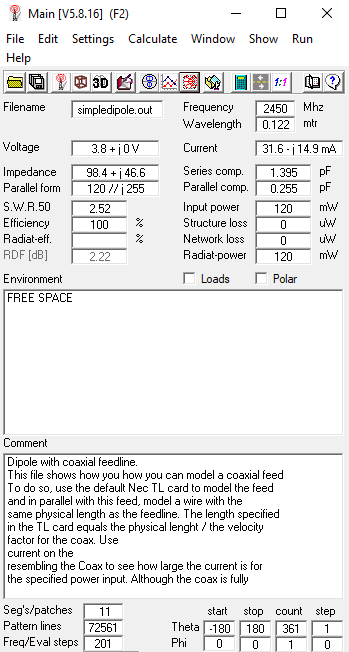
\includegraphics[scale=0.7]{figures/4nec2.PNG}
\caption{Showing the front page of the 4NEC2 program}
\end{figure}

\newpage

\section{Yagi calculator}
The Yagi calculator is also an open source program made by a radio amateur, John Drew\cite{yagical}, with the goal of making it easier to quickly design and build a yagi antenna. This program does not simulate the antenna, but rather uses a template made by years of experimentation in the radio amateur world, even the front page of the program states that, see figure 3.2. The program is capable of calculating the size of the yagi-uda elements, the dimension of the driven element (folded dipole) and the distance between each elements, see section 2.6.7 \textit{Yagi-uda and cross-yagi-uda antennas}. It can calculate the half-power beam width, the gain for each director added. If a coaxial cable is specified the program can calculate the length of the matching stub, to match the yagi antenna to an impedance of $50\Omega$.

\begin{figure}[h!]
\centering
%\hspace*{-2.3cm}
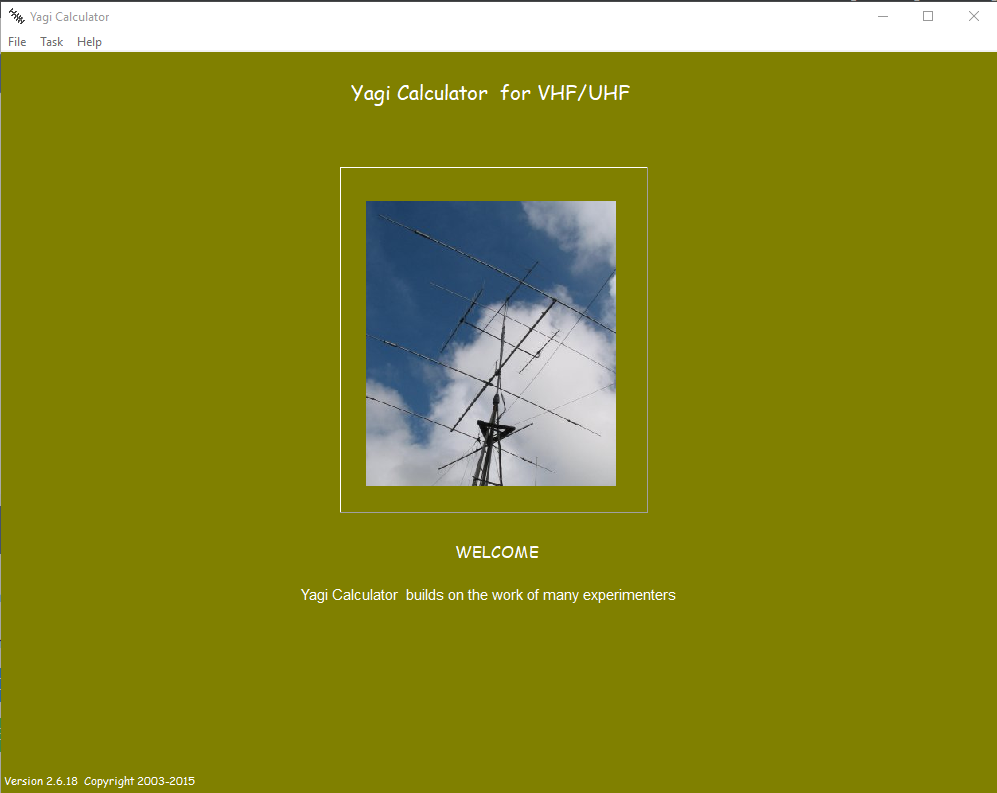
\includegraphics[scale=0.5]{figures/YagiCalculator.PNG}
\caption{Showing the front page of the Yagi calculator program}
\end{figure}

\newpage

\section{Half-wave dipole}
The length of a half-wave dipole, is as the name stated the half of the used wave. Above the wavelength for the center frequency is calculated to be $0.1224meters$, thus the total length of a half-wave dipole is:

\begin{equation}
  Dipole_L = \frac{\lambda}{2} = 0.0609 meters
\end{equation}

Each side elements on the dipole has a length of:

\begin{equation}
  Dipole_E = \frac{\lambda}{4} = 0.0304 meters
\end{equation}

The above result is used in the 4NEC2 program to simulate the antenna, the result from the simulation is in free-space, meaning no ground effects: 

\begin{figure}[h!]
\centering
%\hspace*{-2.3cm}
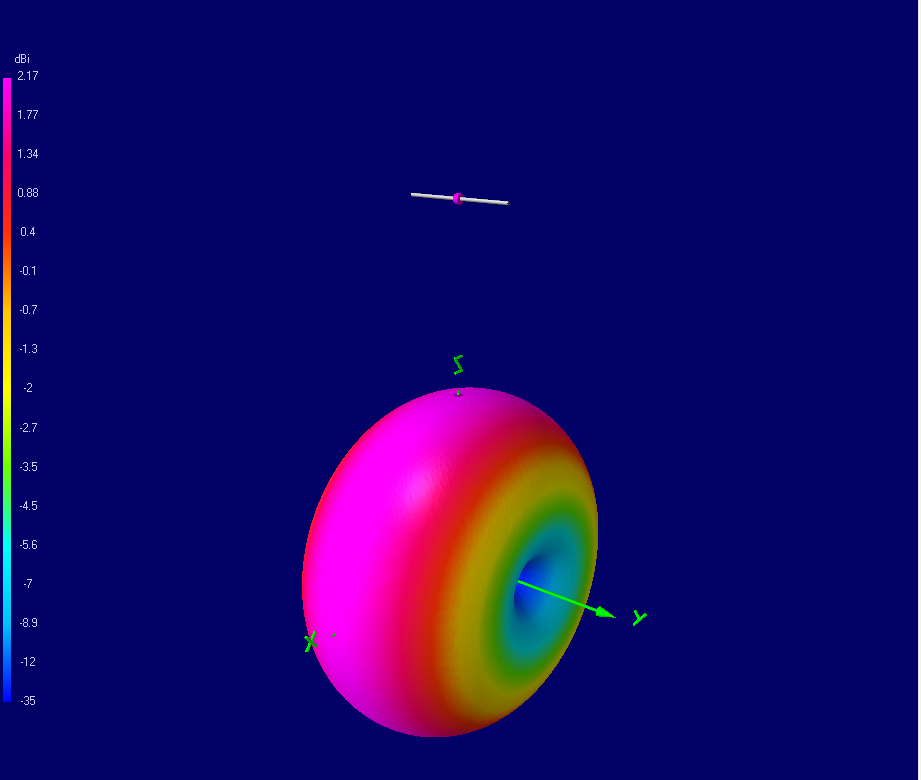
\includegraphics[scale=0.52]{figures/SimulatedDipoleRad.PNG}
\caption{Half-wave dipole antenna 3-dimensional radiation pattern and gain}
\end{figure}

\begin{figure}[h!]
\centering
%\hspace*{-2.3cm}
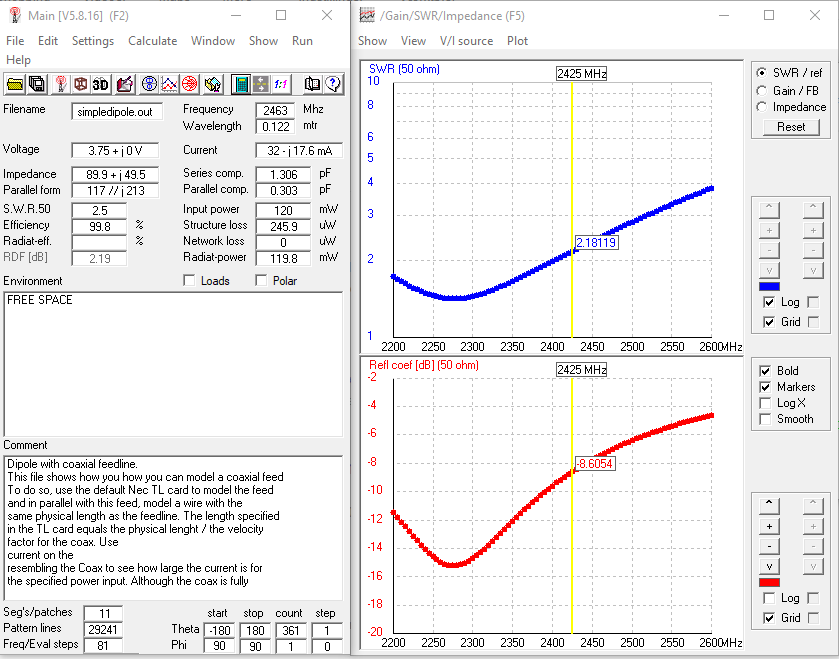
\includegraphics[scale=0.55]{figures/DipoleImpedanceVSWR.PNG}
\caption{Half-wave dipole antenna radiation Impedance and VSWR}
\end{figure}

\begin{figure}[h!]
\centering
%\hspace*{-2.3cm}
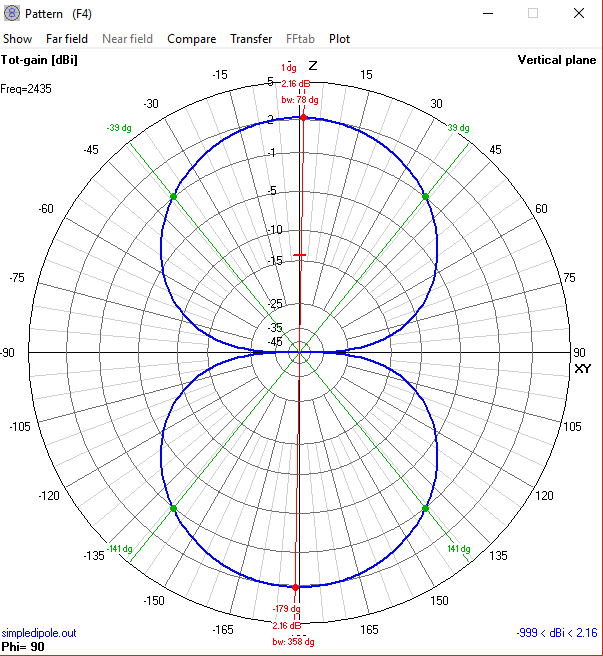
\includegraphics[scale=0.7]{figures/DipoleRadiationPattern.PNG}
\caption{Half-wave dipole antenna 2-dimensional radiation pattern}
\end{figure}

Figure 2.3 shows the radiation pattern in 3-dimensions, it can be observed that the antenna is omnidirectional and has gain of 2.17dBi, which is close to the theoretical 2.15dBi. The impedance is around $89\Omega$, which is slightly higher than the theoretical $73\Omega$, this courses the VSWR to be higher than 1.7 at the center frequency 2463Mhz. Looking at figure 3.4 and table 2.2 it can be observed that a VSWR of 2.5 at the center frequency of 2463Mhz, results in around 20\% reflected power, which is quite high. This is why this type of antenna needs a matching network in order to fully decrease the reflected power. Figure 3.5 show the HPBW to be around \ang{80}.     

\newpage

\section{Sleeved dipole}
The sleeved dipole was simulated by reverse engineering a sleeved dipole bought from china, see figure 2.37. The antenna consists of two pars the sleeved part and the coaxial part, the difference in radius between the two parts is around 2.5mm, which is what can be sen on figure 3.6. This results in some pros and cons, in section 2.6.2 \textit{Sleeved Dipole Antenna} it explained that the thickness of the sleeved part, helps changes the impedance closer to $50\Omega$, which can be seen on figure 3.7, where the impedance is around $52\Omega$, this results in a better VSWR, which is closer to 1.5. A VSWR of 1.5 is around 4\% reflection loss, which is much better than the half-wave dipole, this means that this type of dipole does not need any matching network. The downside of this dipole is the radiation pattern gets disturbed, because the two side elements of the dipole have different radii, as it can be observed on figure 3.6 the gain is around 1.22dBi. 

\begin{figure}[h!]
\centering
%\hspace*{-2.3cm}
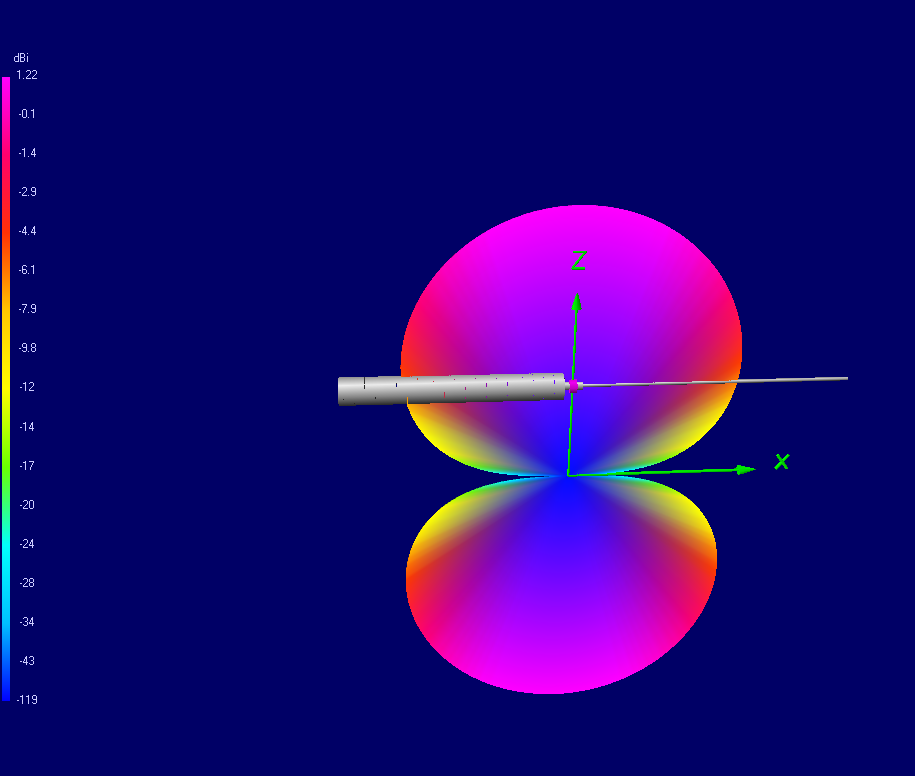
\includegraphics[scale=0.6]{figures/SleevedDipoleRad.PNG}
\caption{Sleeved dipole antenna 3-dimensional radiation pattern and gain}
\end{figure}

\begin{figure}[h!]
\centering
%\hspace*{-2.3cm}
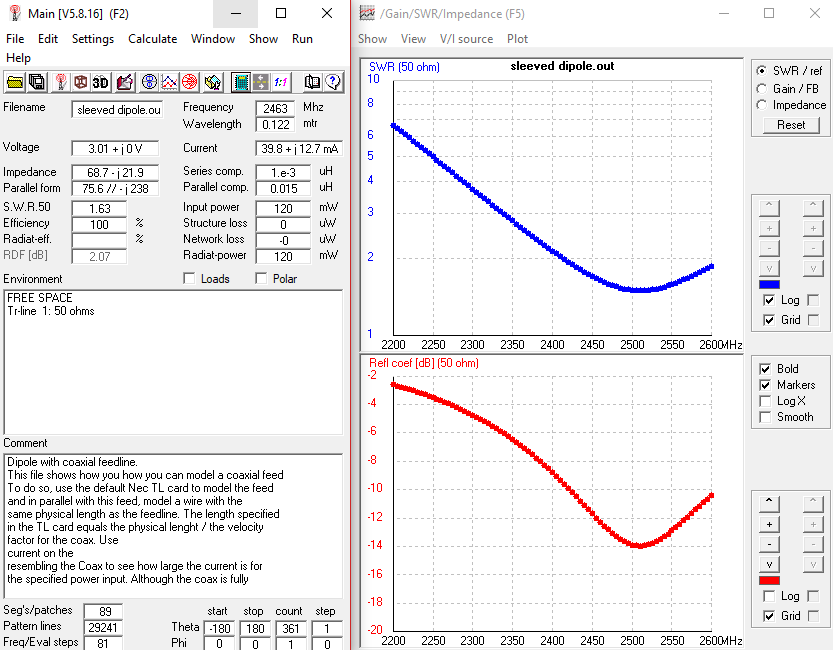
\includegraphics[scale=0.6]{figures/SleevedDipoleImpedanceVSWR.PNG}
\caption{Sleeved dipole  antenna radiation Impedance and VSWR}
\end{figure}

\begin{figure}[h!]
\centering
%\hspace*{-2.3cm}
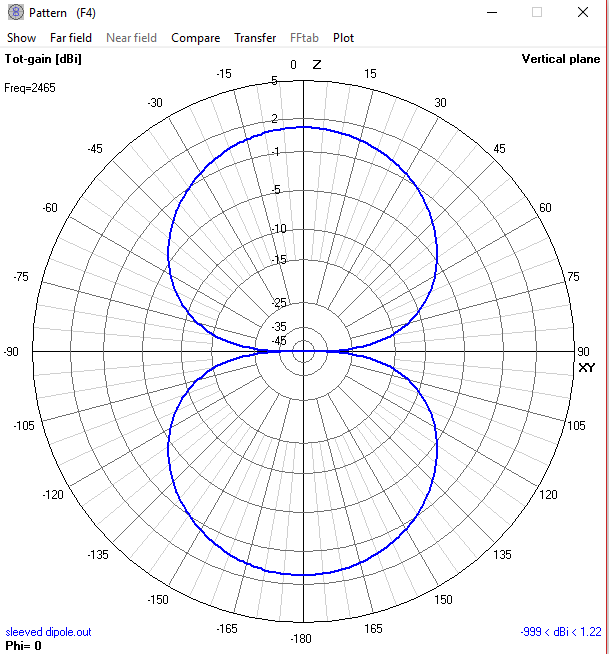
\includegraphics[scale=0.60]{figures/SleevedDipoleRadiationPatternPNG.PNG}
\caption{Sleeved dipole  antenna 2-dimensional radiation pattern}
\end{figure}

\newpage

\section{Quarter-wave monopol}
Figure 2.40 shows that the driven element of a quarter-wave monopol antenna is $\frac{\lambda}{4}$, but also for the radials- the 4 side pin sticking out. That is the same length as the results from equation (3.4). The quarter-wave monopol antenna is essentially a monopol antenna with its own ground, this antenna was simulated in free-space resulting in a dipole radiation shape if the antenna get closer to a ground plane, the shape will change to look something like the figure 2.39. The purpose of the radials, is to simulate a ground plane, and to control the impedance of the antenna. By bending the radials 30 to 40 degrees the impedance of the antenna will be closer to $50\Omega$, see figure 3.10. On figure 3.9 the radials has been bent by about 30 degrees, the gain of this antenna is close to a dipole, depending on how well the ground plane is constructed the gain is around 1.5 to 2.15 dBi. Furthermore, figure 3.11 shows that the HPBW is around 90 degrees.      

\begin{figure}[h!]
%\centering
\hspace*{-1.5cm}
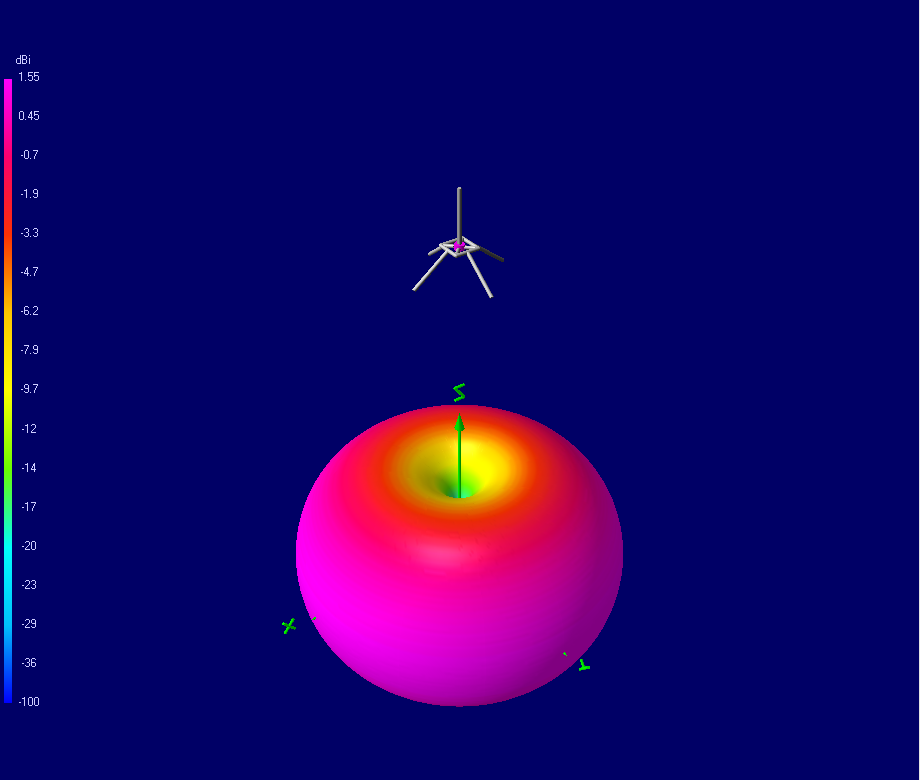
\includegraphics[scale=0.7]{figures/QuaterwaveMonopolAntennaRad.PNG}
\caption{Quarter-wave monopol antenna 3-dimensional radiation pattern and gain}
\end{figure}

\begin{figure}[h!]
\centering
%\hspace*{-2.3cm}
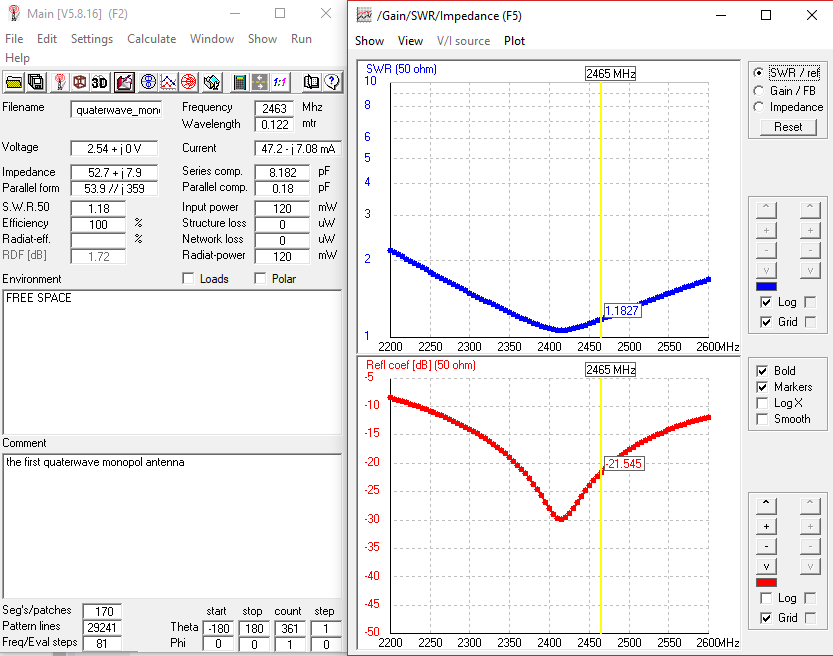
\includegraphics[scale=0.60]{figures/QuaterwaveMonopolAntennaImpedanceVSWR.PNG}
\caption{Quarter-wave monopol  antenna radiation Impedance and VSWR}
\end{figure}

\begin{figure}[h!]
\centering
%\hspace*{-2.3cm}
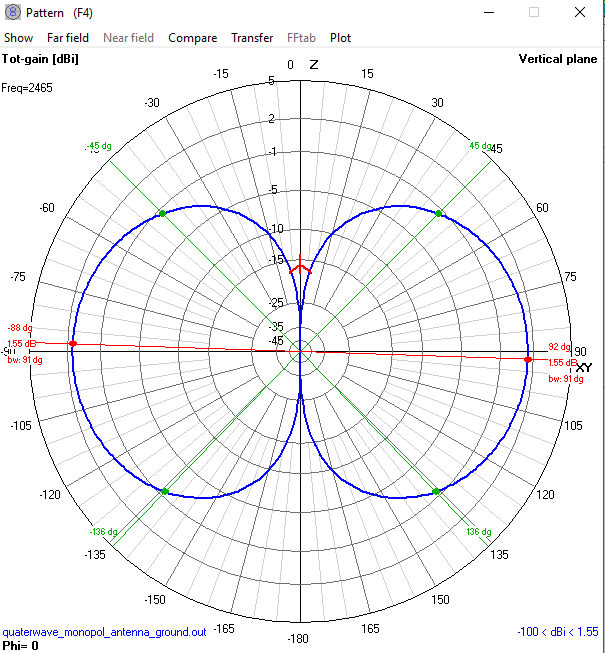
\includegraphics[scale=0.60]{figures/QuaterwaveMonopolAntennaRadiationPattern.PNG}
\caption{Quarter-wave monopol  antenna 2-dimensional radiation pattern}
\end{figure}

\newpage

% show the simulations and results
\section{Helical}
From the theory described in section 2.6.5 \textit{Helical antenna} it is possible to calculate how the helical antenna should look like. For this MATLAB\cite{MatLab} was used to setup all the parameters and formulas, written in the theory. See the code in appendix F. The output of the code is seen below on table 3.1

\begin{table}[h!]
\centering
\begin{tabular}{|l|l|l|}
\hline
Name      & Value              & Unit                   \\ \hline
freq      & 2450000000         & Hz                     \\ \hline
lambda    & 0.122364268571429  & Meters                 \\ \hline
N         & 25                 & n/A                    \\ \hline
C         & 0.128482482        & Meters                 \\ \hline
ans       & 1                  & Logical                \\ \hline
ans       & 1                  & Logical                \\ \hline
D         & 0.0408972442220309 & Meters                 \\ \hline
f1        & 1754385964.91228   & Hz                     \\ \hline
f2        & 3111111111.11111   & Hz                     \\ \hline
fc        & 2432748538.0117    & Hz                     \\ \hline
FBW       & 55.7692307692308   & Percentage             \\ \hline
R         & 0.122364268571429  & Meters                 \\ \hline
ans       & 1                  & Logical                \\ \hline
ans       & 1                  & Logical                \\ \hline
S         & 0.0307908657307696 & Meters                 \\ \hline
S\_g      & 0.0146837122285714 & Meters                 \\ \hline
L         & 0.132120496492144  & Meters                 \\ \hline
NL        & 3.3030124123036    & Meters                 \\ \hline
totLength & 0.769771643269241  & Meters                 \\ \hline
HPBW      & 19.7451482824545   & Degrees                \\ \hline
Z0        & 147                & $\Omega$               \\ \hline
GARRL     & 20.2108588815563   & dBi                    \\ \hline
GWIKI     & 20.1717714721131   & dBi                    \\ \hline
\end{tabular}
\caption{Matlab output code for all the parameters for a helical antenna, see Appendix F and section 2.6.5 \textit{Helical antenna} for further information}
\end{table}

The helical antenna was simulated using the parameters in table 3.1. Since it is really hard to graphically draw a circle, in the 4NEC2 program, for the helical ground plane, instead the antenna was simulated above perfect ground. Furthermore the simulation does not include the Heckers transformer, see figure 2.44,  used to lower the impedance to $50\Omega$. Once the antenna is build, testing it with a VVIA should be done before and after adding the Heckers transformer, thus a reference can be made between the physical antenna and the simulated antenna.


Figure 3.12 show that the antenna is indeed a high gain antenna, with a main peak of about 17 dBi, around 3 dBi lower than the theoretically value, see table 3.1, GARRL and GWIKI. The reason for this is lack of proper ground plane reflection, as one can observe there are too many big side lobes, which "steals" the RF energy from the main peak. A paper exists to combat this problem, see reference\cite{HelicalGoodGround}, it explains how to build a proper ground plane for the helical antenna.  
\begin{figure}[h!]
\centering
%\hspace*{-1cm}
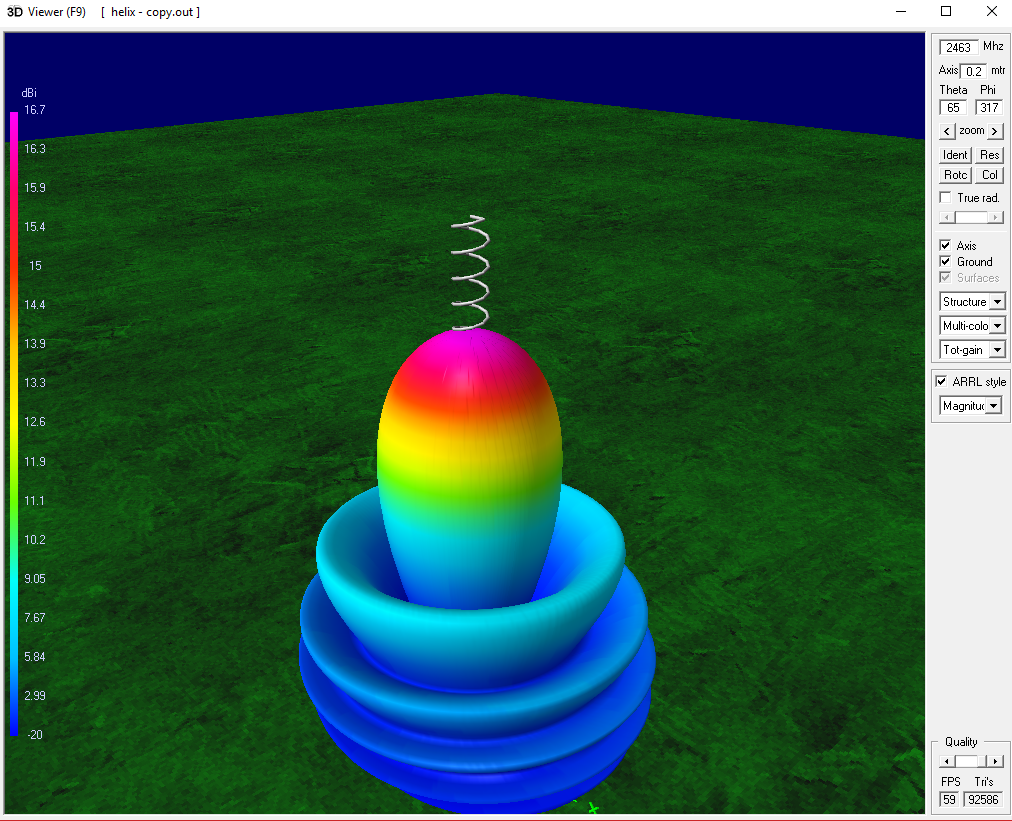
\includegraphics[scale=0.55]{figures/HelicalAntennaRad.PNG}
\caption{Helical antenna 3-dimensional radiation pattern and gain}
\end{figure}

Table 3.1 states that the FBW is around 55\% witch means that the helical antenna a wideband antenna, this can also be observed on figure 3.13 where the VSWR is more linear than any of the other antennas. Once the Heckers Transformer has been added the VSWR will further drop, but still stay wide banded. The impedance of the Antenna is simulated to be around $116\Omega$, which is around $31\Omega$ less than the calculated impedance, seen on table 3.1 $Z_0$. Figure 3.14 shows the radiation pattern on a 2-dimensional plane, what can be observed is the green lines, these are the HPBW simulated to be \ang{24}, which is not that far away from what is calculated on table 3.1 HPBW around \ang{20}.    

\begin{figure}[h!]
\centering
%\hspace*{-2.3cm}
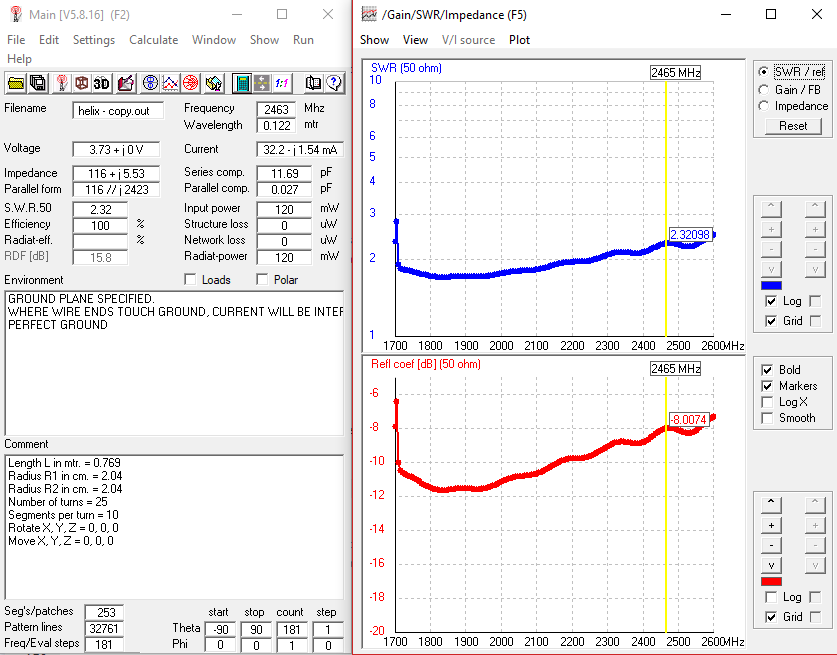
\includegraphics[scale=0.57]{figures/HelicalAntennaImpedanceVSWR.PNG}
\caption{Helical antenna radiation Impedance and VSWR}
\end{figure}

\begin{figure}[h!]
\centering
%\hspace*{-2.3cm}
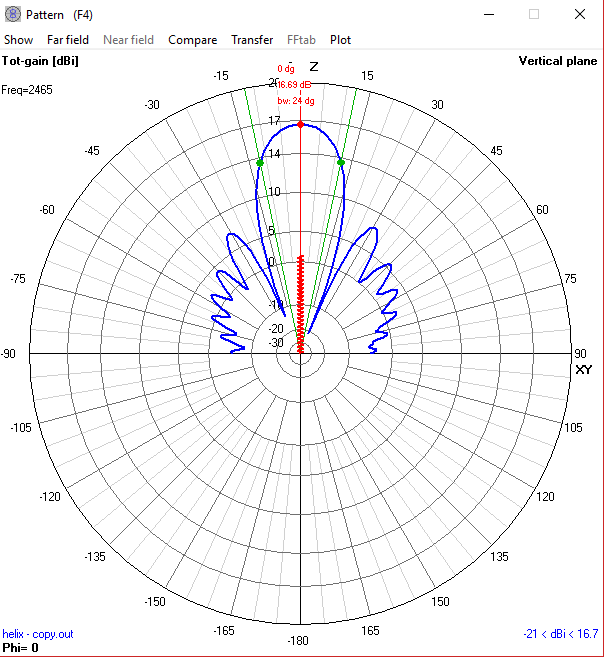
\includegraphics[scale=0.57]{figures/HelicalAntennaRadiationPattern.PNG}
\caption{Helical antenna 2-dimensional radiation pattern}
\end{figure}

\newpage

\section{Yagi-uda and cross-yagi-uda}
The calculation for the yagi-uda and cross-yagi-uda antenna, was done by using the \textit{Yagi Calculator}, see section 3.2 \textit{Yagi Calculator}. This program is easy to use, by just adding the needed values the program will output basically everything need to build a yagi-uda antenna. The program only calculates for a yagi-uda and not for a cross yagi-uda. Section 2.6.7 \textit{Yagi-uda and cross-yagi-uda antennas} describes the theory behind cross-yagi-uda antanna. with the theory, and the calculator it is possible to build a cross-yagi-uda antenna.

Once the variables has been inserted, the results will be available, see figure 3.15 and appendix G.

\begin{figure}[h!]
\centering
%\hspace*{-2.3cm}
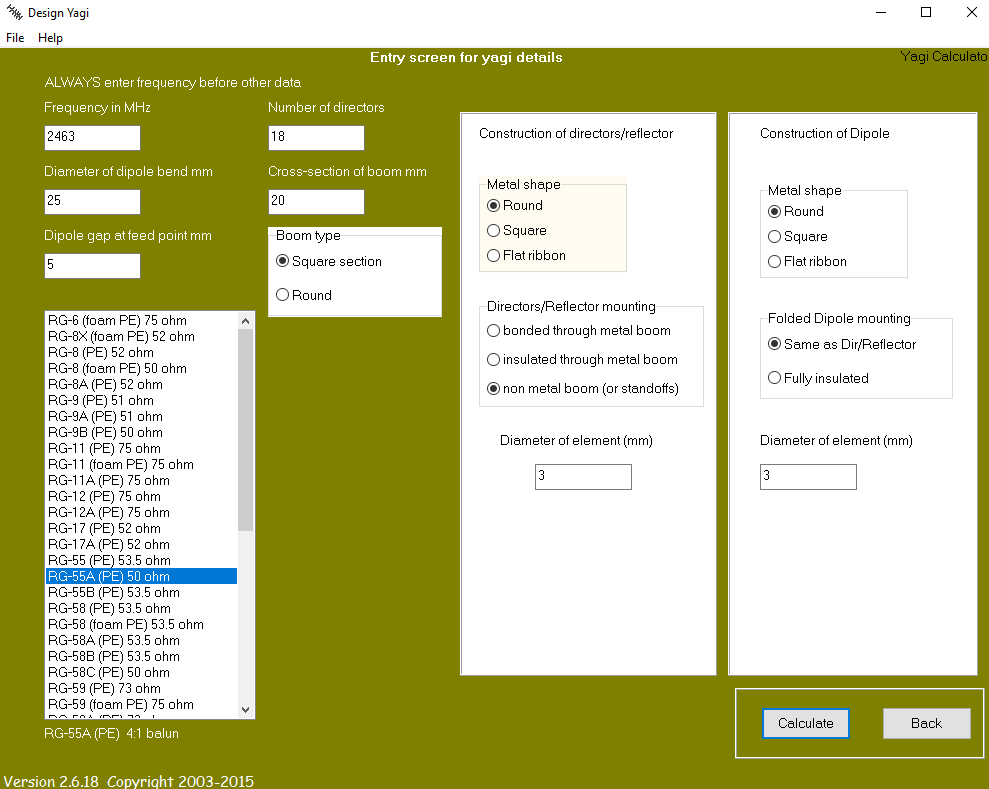
\includegraphics[scale=0.60]{figures/YagiCalculatorVeriables.PNG}
\caption{Variables inserted in the calculator}
\end{figure}

After using the calculator an analyzing the data, it was obvious that in order to build a cross-yagi-uda antenna in the high frequency of 2463MHz, the directors elements of the yagi antennas would end up intersecting each other, making it very complex and time consuming to construct such an antenna, therefore the helical yagi-uda and cross-yagi-uda antennas was excluded in favor for using an helical antenna. This is why it will no make sense to show the simulation for these two antennas. If for some reason the reader wants to build his own yagi-uda or cross-yagi-uda antenna, this reference\cite{StudyAndDesignYagiCrossAntenna}\ is good to use as guideline. The authors of the paper actually used 4NEC2 program to simulate the antennas, by using their results the reader should have the necessary knowledge to build the antennas. For simplicity reasons, a cheap yagi-uda antenna was bought from china to use as reference against the helical antenna.  

\section{Partial conclusion}
Since the ground system has to have an antenna that is circular polarized only two antennas can be used on the ground. It is either a cross-yagi-uda or a helical antenna. Looking into the complexity and price  of building a cross-yagi-uda antenna compared to a helical antenna, it is clear that the favor goes to the helical antenna. When it comes to the antennas mounted inside the rocket, either the sleeved dipole or the quarter-wave monopol antenna will fit the match, since by default they are matched to $50\Omega$, without the need of external matching networks, assuming that the simulation is correct. It can therefore be concluded, that the best antenna to build, for the ground system, is the helical antenna. For the rocket it is either the quarter-wave monopol or sleeved antenna, depending on which one of those is easiest to mount in the rocket.  

